\subsection{Zbiór "Iris"}
    \begin{figure}[H]
        \center
        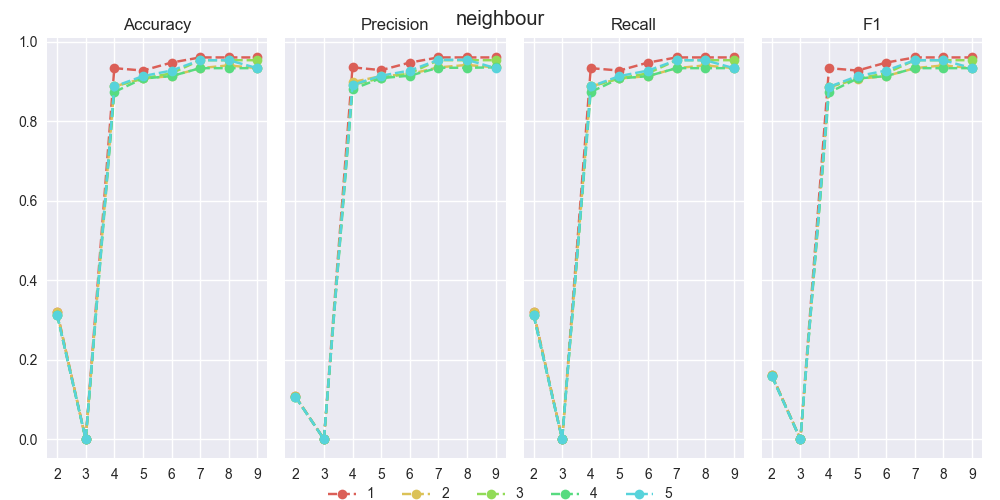
\includegraphics[width=\textwidth]{resources/plots/iris_KFold_neighbour.png}
        \caption{Wykres wartości miar dla zbioru "Iris" dla różnej liczby sąsiadów (kroswalidacja zwykła).}
    \end{figure}

    \begin{figure}[H]
        \center
        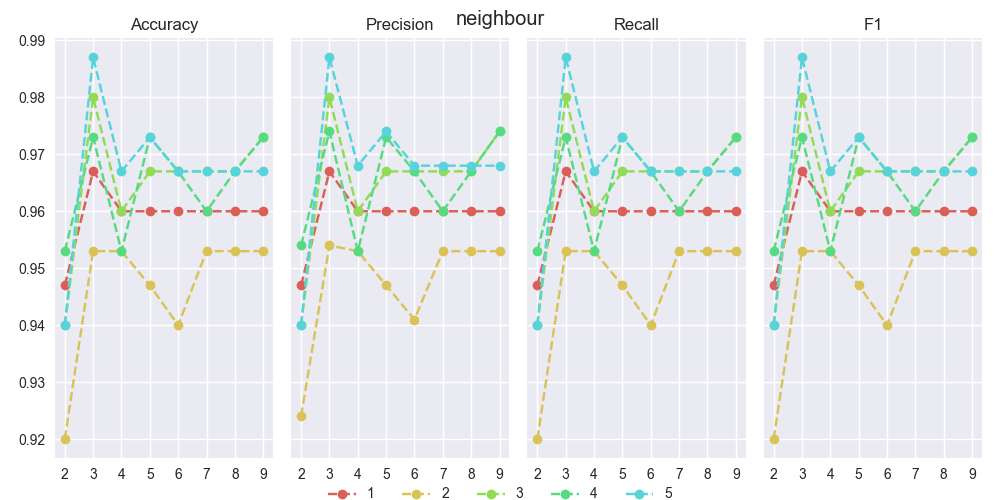
\includegraphics[width=\textwidth]{resources/plots/iris_StratifiedKFold_neighbour.png}
        \caption{Wykres wartości miar dla zbioru "Iris" dla różnej liczby sąsiadów (kroswalidacja stratyfikowana).}
    \end{figure}

    
\begin{table}[H]
    \begin{tabular}{c|c|cccccccc}
       \multirow{2}{*}{Wartość parametru} & \multirow{2}{*}{Metryka} & \multicolumn{8}{|c|}{Kroswalidacja} \\
         & & K = 2 & K = 3 & K = 4 & K = 5 & K = 6 & K = 7 & K = 8 & K = 9 \\ \hline
         1&Accuracy&0.32& 0.0& 0.933& 0.927& 0.947& 0.96& 0.96& 0.96\\ \hline
1&Precision&0.108& 0.0& 0.935& 0.928& 0.947& 0.96& 0.96& 0.96\\ \hline
1&Recall&0.32& 0.0& 0.933& 0.927& 0.947& 0.96& 0.96& 0.96\\ \hline
1&F1&0.162& 0.0& 0.933& 0.927& 0.947& 0.96& 0.96& 0.96\\ \hline
2&Accuracy&0.32& 0.0& 0.887& 0.907& 0.913& 0.933& 0.94& 0.933\\ \hline
2&Precision&0.108& 0.0& 0.898& 0.913& 0.918& 0.935& 0.941& 0.935\\ \hline
2&Recall&0.32& 0.0& 0.887& 0.907& 0.913& 0.933& 0.94& 0.933\\ \hline
2&F1&0.162& 0.0& 0.885& 0.906& 0.913& 0.933& 0.94& 0.933\\ \hline
3&Accuracy&0.313& 0.0& 0.887& 0.907& 0.92& 0.953& 0.953& 0.953\\ \hline
3&Precision&0.107& 0.0& 0.891& 0.908& 0.92& 0.953& 0.953& 0.953\\ \hline
3&Recall&0.313& 0.0& 0.887& 0.907& 0.92& 0.953& 0.953& 0.953\\ \hline
3&F1&0.159& 0.0& 0.886& 0.907& 0.92& 0.953& 0.953& 0.953\\ \hline
4&Accuracy&0.313& 0.0& 0.873& 0.907& 0.913& 0.933& 0.933& 0.933\\ \hline
4&Precision&0.107& 0.0& 0.88& 0.908& 0.914& 0.934& 0.934& 0.935\\ \hline
4&Recall&0.313& 0.0& 0.873& 0.907& 0.913& 0.933& 0.933& 0.933\\ \hline
4&F1&0.159& 0.0& 0.872& 0.907& 0.913& 0.933& 0.933& 0.933\\ \hline
5&Accuracy&0.313& 0.0& 0.887& 0.913& 0.927& 0.953& 0.953& 0.933\\ \hline
5&Precision&0.107& 0.0& 0.891& 0.914& 0.927& 0.954& 0.954& 0.933\\ \hline
5&Recall&0.313& 0.0& 0.887& 0.913& 0.927& 0.953& 0.953& 0.933\\ \hline
5&F1&0.159& 0.0& 0.886& 0.913& 0.927& 0.953& 0.953& 0.933 \\ \hline
    \end{tabular}
    \caption{Wartości miar dla zbioru "Iris" dla różnej liczby sąsiadów (kroswalidacja zwykła).}
\end{table}
    
    
\begin{table}[H]
    \begin{tabular}{c|c|cccccccc}
       \multirow{2}{*}{Wartość parametru} & \multirow{2}{*}{Metryka} & \multicolumn{8}{|c|}{Kroswalidacja} \\
         & & K = 2 & K = 3 & K = 4 & K = 5 & K = 6 & K = 7 & K = 8 & K = 9 \\ \hline
         1&Accuracy&0.947& 0.967& 0.96& 0.96& 0.96& 0.96& 0.96& 0.96\\ \hline
1&Precision&0.947& 0.967& 0.96& 0.96& 0.96& 0.96& 0.96& 0.96\\ \hline
1&Recall&0.947& 0.967& 0.96& 0.96& 0.96& 0.96& 0.96& 0.96\\ \hline
1&F1&0.947& 0.967& 0.96& 0.96& 0.96& 0.96& 0.96& 0.96\\ \hline
2&Accuracy&0.92& 0.953& 0.953& 0.947& 0.94& 0.953& 0.953& 0.953\\ \hline
2&Precision&0.924& 0.954& 0.953& 0.947& 0.941& 0.953& 0.953& 0.953\\ \hline
2&Recall&0.92& 0.953& 0.953& 0.947& 0.94& 0.953& 0.953& 0.953\\ \hline
2&F1&0.92& 0.953& 0.953& 0.947& 0.94& 0.953& 0.953& 0.953\\ \hline
3&Accuracy&0.94& 0.98& 0.96& 0.967& 0.967& 0.967& 0.967& 0.973\\ \hline
3&Precision&0.94& 0.98& 0.96& 0.967& 0.967& 0.967& 0.967& 0.974\\ \hline
3&Recall&0.94& 0.98& 0.96& 0.967& 0.967& 0.967& 0.967& 0.973\\ \hline
3&F1&0.94& 0.98& 0.96& 0.967& 0.967& 0.967& 0.967& 0.973\\ \hline
4&Accuracy&0.953& 0.973& 0.953& 0.973& 0.967& 0.96& 0.967& 0.973\\ \hline
4&Precision&0.954& 0.974& 0.953& 0.973& 0.967& 0.96& 0.967& 0.974\\ \hline
4&Recall&0.953& 0.973& 0.953& 0.973& 0.967& 0.96& 0.967& 0.973\\ \hline
4&F1&0.953& 0.973& 0.953& 0.973& 0.967& 0.96& 0.967& 0.973\\ \hline
5&Accuracy&0.94& 0.987& 0.967& 0.973& 0.967& 0.967& 0.967& 0.967\\ \hline
5&Precision&0.94& 0.987& 0.968& 0.974& 0.968& 0.968& 0.968& 0.968\\ \hline
5&Recall&0.94& 0.987& 0.967& 0.973& 0.967& 0.967& 0.967& 0.967\\ \hline
5&F1&0.94& 0.987& 0.967& 0.973& 0.967& 0.967& 0.967& 0.967 \\ \hline
    \end{tabular}
    \caption{Wartości miar dla zbioru "Iris" dla różnej liczby sąsiadów (kroswalidacja stratyfikowana).}
\end{table}
    

    \pagebreak

    \begin{figure}[H]
        \center
        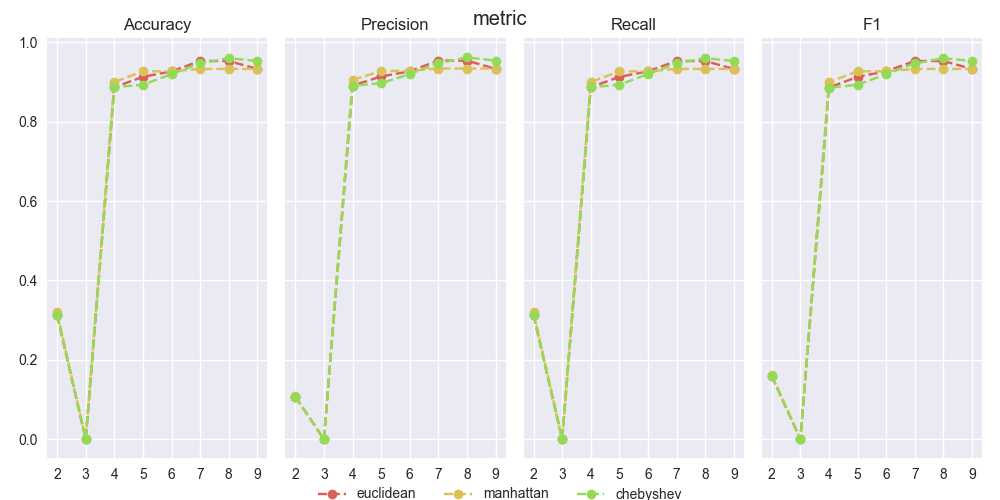
\includegraphics[width=\textwidth]{resources/plots/iris_KFold_metric.png}
        \caption{Wykres wartości miar dla zbioru "Iris" dla różnych metryk odległości (kroswalidacja zwykła).}
    \end{figure}

    \begin{figure}[H]
        \center
        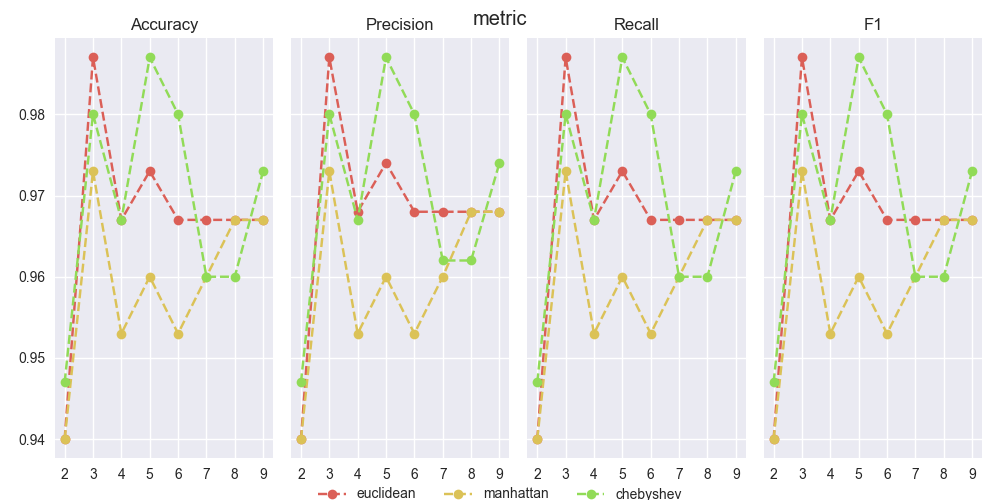
\includegraphics[width=\textwidth]{resources/plots/iris_StratifiedKFold_metric.png}
        \caption{Wykres wartości miar dla zbioru "Iris" dla różnych metryk odległości (kroswalidacja stratyfikowana).}
    \end{figure}

    
\begin{table}[H]
    \begin{tabular}{c|c|cccccccc}
       \multirow{2}{*}{Wartość parametru} & \multirow{2}{*}{Metryka} & \multicolumn{8}{|c|}{Kroswalidacja} \\
         & & K = 2 & K = 3 & K = 4 & K = 5 & K = 6 & K = 7 & K = 8 & K = 9 \\ \hline
         euclidean&Accuracy&0.313& 0.0& 0.887& 0.913& 0.927& 0.953& 0.953& 0.933\\ \hline
euclidean&Precision&0.107& 0.0& 0.891& 0.914& 0.927& 0.954& 0.954& 0.933\\ \hline
euclidean&Recall&0.313& 0.0& 0.887& 0.913& 0.927& 0.953& 0.953& 0.933\\ \hline
euclidean&F1&0.159& 0.0& 0.886& 0.913& 0.927& 0.953& 0.953& 0.933\\ \hline
manhattan&Accuracy&0.32& 0.0& 0.9& 0.927& 0.927& 0.933& 0.933& 0.933\\ \hline
manhattan&Precision&0.108& 0.0& 0.905& 0.928& 0.928& 0.934& 0.934& 0.934\\ \hline
manhattan&Recall&0.32& 0.0& 0.9& 0.927& 0.927& 0.933& 0.933& 0.933\\ \hline
manhattan&F1&0.162& 0.0& 0.9& 0.927& 0.927& 0.933& 0.933& 0.933\\ \hline
chebyshev&Accuracy&0.313& 0.0& 0.887& 0.893& 0.92& 0.947& 0.96& 0.953\\ \hline
chebyshev&Precision&0.107& 0.0& 0.891& 0.897& 0.92& 0.947& 0.962& 0.954\\ \hline
chebyshev&Recall&0.313& 0.0& 0.887& 0.893& 0.92& 0.947& 0.96& 0.953\\ \hline
chebyshev&F1&0.159& 0.0& 0.886& 0.893& 0.92& 0.947& 0.96& 0.953 \\ \hline
    \end{tabular}
    \caption{Wartości miar dla zbioru "Iris" dla różnych metryk odległości (kroswalidacja zwykła).}
\end{table}
    
    
\begin{table}[H]
    \begin{tabular}{c|c|cccccccc}
       \multirow{2}{*}{Wartość parametru} & \multirow{2}{*}{Metryka} & \multicolumn{8}{|c|}{Kroswalidacja} \\
         & & K = 2 & K = 3 & K = 4 & K = 5 & K = 6 & K = 7 & K = 8 & K = 9 \\ \hline
         euclidean&Accuracy&0.94& 0.987& 0.967& 0.973& 0.967& 0.967& 0.967& 0.967\\ \hline
euclidean&Precision&0.94& 0.987& 0.968& 0.974& 0.968& 0.968& 0.968& 0.968\\ \hline
euclidean&Recall&0.94& 0.987& 0.967& 0.973& 0.967& 0.967& 0.967& 0.967\\ \hline
euclidean&F1&0.94& 0.987& 0.967& 0.973& 0.967& 0.967& 0.967& 0.967\\ \hline
manhattan&Accuracy&0.94& 0.973& 0.953& 0.96& 0.953& 0.96& 0.967& 0.967\\ \hline
manhattan&Precision&0.94& 0.973& 0.953& 0.96& 0.953& 0.96& 0.968& 0.968\\ \hline
manhattan&Recall&0.94& 0.973& 0.953& 0.96& 0.953& 0.96& 0.967& 0.967\\ \hline
manhattan&F1&0.94& 0.973& 0.953& 0.96& 0.953& 0.96& 0.967& 0.967\\ \hline
chebyshev&Accuracy&0.947& 0.98& 0.967& 0.987& 0.98& 0.96& 0.96& 0.973\\ \hline
chebyshev&Precision&0.947& 0.98& 0.967& 0.987& 0.98& 0.962& 0.962& 0.974\\ \hline
chebyshev&Recall&0.947& 0.98& 0.967& 0.987& 0.98& 0.96& 0.96& 0.973\\ \hline
chebyshev&F1&0.947& 0.98& 0.967& 0.987& 0.98& 0.96& 0.96& 0.973 \\ \hline
    \end{tabular}
    \caption{Wartości miar dla zbioru "Iris" dla różnych metryk odległości (kroswalidacja stratyfikowana).}
\end{table}
    

    \pagebreak

    \begin{figure}[H]
        \center
        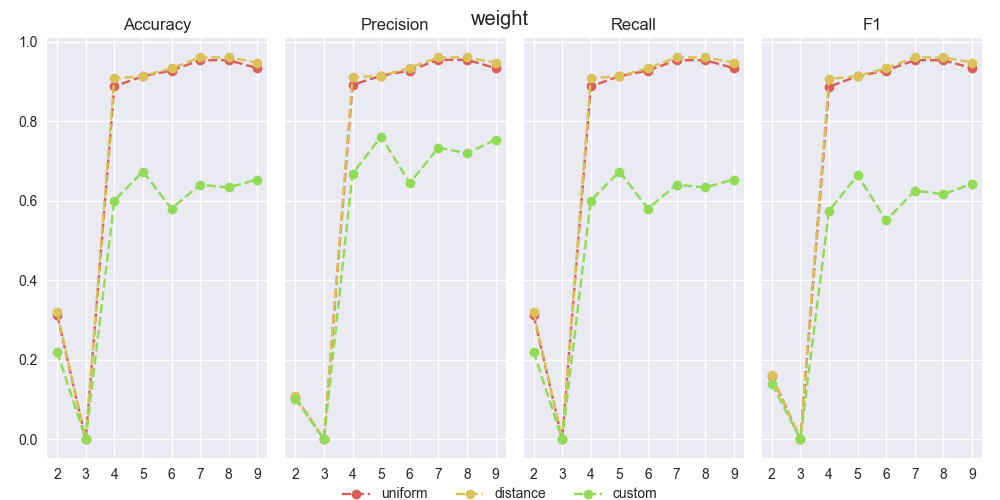
\includegraphics[width=\textwidth]{resources/plots/iris_KFold_weight.png}
        \caption{Wykres wartości miar dla zbioru "Iris" dla różnych sposobów głosowania (kroswalidacja zwykła).}
    \end{figure}

    \begin{figure}[H]
        \center
        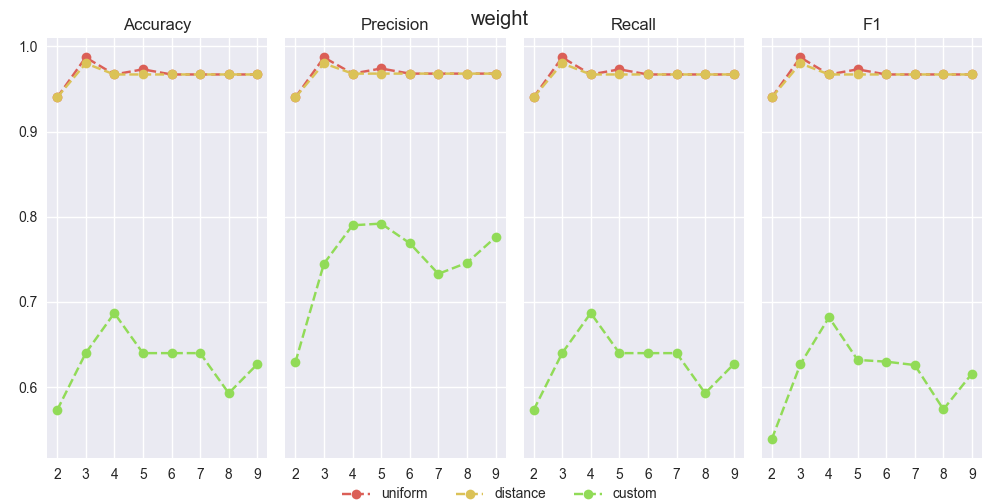
\includegraphics[width=\textwidth]{resources/plots/iris_StratifiedKFold_weight.png}
        \caption{Wykres wartości miar dla zbioru "Iris" dla różnych sposobów głosowania (kroswalidacja stratyfikowana).}
    \end{figure}

    
\begin{table}[H]
    \begin{tabular}{c|c|cccccccc}
       \multirow{2}{*}{Wartość parametru} & \multirow{2}{*}{Metryka} & \multicolumn{8}{|c|}{Kroswalidacja} \\
         & & K = 2 & K = 3 & K = 4 & K = 5 & K = 6 & K = 7 & K = 8 & K = 9 \\ \hline
         uniform&Accuracy&0.313& 0.0& 0.887& 0.913& 0.927& 0.953& 0.953& 0.933\\ \hline
uniform&Precision&0.107& 0.0& 0.891& 0.914& 0.927& 0.954& 0.954& 0.933\\ \hline
uniform&Recall&0.313& 0.0& 0.887& 0.913& 0.927& 0.953& 0.953& 0.933\\ \hline
uniform&F1&0.159& 0.0& 0.886& 0.913& 0.927& 0.953& 0.953& 0.933\\ \hline
distance&Accuracy&0.32& 0.0& 0.907& 0.913& 0.933& 0.96& 0.96& 0.947\\ \hline
distance&Precision&0.108& 0.0& 0.91& 0.914& 0.934& 0.96& 0.96& 0.947\\ \hline
distance&Recall&0.32& 0.0& 0.907& 0.913& 0.933& 0.96& 0.96& 0.947\\ \hline
distance&F1&0.162& 0.0& 0.906& 0.913& 0.933& 0.96& 0.96& 0.947\\ \hline
custom&Accuracy&0.233& 0.0& 0.607& 0.567& 0.613& 0.593& 0.673& 0.627\\ \hline
custom&Precision&0.112& 0.0& 0.681& 0.691& 0.699& 0.729& 0.803& 0.726\\ \hline
custom&Recall&0.233& 0.0& 0.607& 0.567& 0.613& 0.593& 0.673& 0.627\\ \hline
custom&F1&0.152& 0.0& 0.583& 0.535& 0.591& 0.573& 0.67& 0.61 \\ \hline
    \end{tabular}
    \caption{Wartości miar dla zbioru "Iris" dla różnych sposobów głosowania (kroswalidacja zwykła).}
\end{table}
    
    
\begin{table}[H]
    \begin{tabular}{c|c|cccccccc}
       \multirow{2}{*}{Wartość parametru} & \multirow{2}{*}{Metryka} & \multicolumn{8}{|c|}{Kroswalidacja} \\
         & & K = 2 & K = 3 & K = 4 & K = 5 & K = 6 & K = 7 & K = 8 & K = 9 \\ \hline
         uniform&Accuracy&0.94& 0.987& 0.967& 0.973& 0.967& 0.967& 0.967& 0.967\\ \hline
uniform&Precision&0.94& 0.987& 0.968& 0.974& 0.968& 0.968& 0.968& 0.968\\ \hline
uniform&Recall&0.94& 0.987& 0.967& 0.973& 0.967& 0.967& 0.967& 0.967\\ \hline
uniform&F1&0.94& 0.987& 0.967& 0.973& 0.967& 0.967& 0.967& 0.967\\ \hline
distance&Accuracy&0.94& 0.98& 0.967& 0.967& 0.967& 0.967& 0.967& 0.967\\ \hline
distance&Precision&0.94& 0.98& 0.968& 0.968& 0.968& 0.968& 0.968& 0.968\\ \hline
distance&Recall&0.94& 0.98& 0.967& 0.967& 0.967& 0.967& 0.967& 0.967\\ \hline
distance&F1&0.94& 0.98& 0.967& 0.967& 0.967& 0.967& 0.967& 0.967\\ \hline
custom&Accuracy&0.653& 0.573& 0.687& 0.647& 0.62& 0.68& 0.7& 0.673\\ \hline
custom&Precision&0.769& 0.665& 0.778& 0.752& 0.75& 0.764& 0.795& 0.786\\ \hline
custom&Recall&0.653& 0.573& 0.687& 0.647& 0.62& 0.68& 0.7& 0.673\\ \hline
custom&F1&0.644& 0.544& 0.675& 0.634& 0.605& 0.67& 0.692& 0.668 \\ \hline
    \end{tabular}
    \caption{Wartości miar dla zbioru "Iris" dla różnych sposobów głosowania (kroswalidacja stratyfikowana).}
\end{table}
    